\documentclass{beamer}

\usepackage[utf8]{inputenc}
\usepackage{default}

\setbeamertemplate{navigation symbols}{}

\usetheme{Ilmenau}
\setbeamercolor{frametitle}{fg=black,bg=white}
\setbeamercolor{title}{fg=black,bg=red!75!black}



\beamersetuncovermixins{\opaqueness<1>{25}}{\opaqueness<2->{15}}
\begin{document}
\title{The basics of the DMC code}
\author{Jørgen Høgberget}
\date{} 

\begin{frame}
\titlepage
\end{frame}

\begin{frame}\frametitle{Table of contents}\tableofcontents
\end{frame} 


\section{Aims and limitations} 
\begin{frame}\frametitle{What can it do?} 

\begin{alertblock}{Quantities of interest}
\begin{itemize}
 \item Ground state energies and densities.
 \item Energy distributions.
\end{itemize}
\end{alertblock}

\pause
\begin{alertblock}{Implemented Systems}
\begin{itemize}
\item Harmonic oscillator systems (2D, 3D, doublewells)
\item Atomic systems (Atoms, homonuclear diatomic molecules)
\end{itemize}
\end{alertblock}

\end{frame}

\begin{frame}\frametitle{Underlying goals and assumptions}

\begin{alertblock}{In a nutshell}
 \textit{Ab-initio}, Efficiency, Transparency
\end{alertblock}

\pause

\begin{alertblock}{Specifics: Assumptions}
\begin{itemize}
 \item Single Slater-determinant ansatz.
 \item Single-parameter Jastrow correlation function.
\end{itemize}
\end{alertblock}

\end{frame}


\begin{frame}\frametitle{Why ab-initio?}

\begin{itemize}
 \item Avoid self-consistency in multi-scale modelling.
 \pause\item System acts independent of our aims of the computation - nature is not influenced by our intentions.
 \pause\item Fundamental modelling: High academic eigenvalue.
 \pause\item Downside: It is harder to solve equations when you cannot assume to know the answer (even if you do).
\end{itemize}

\end{frame}

\begin{frame}\frametitle{Efficiency vs. generalization and precision}

The precision of DMC (given a model Hamiltonian) is, to first approximation, limited by one thing: \textbf{The trial wave function}.

\pause
\vspace{0.5cm}

\begin{equation*}
 \text{SP-basis} \quad \to \quad \text{Det. Basis} \quad \to \quad \text{Combine Determinants}
\end{equation*}


\end{frame}

\begin{frame}\frametitle{Efficiency vs. generalization and precision}

The precision of DMC (given a model Hamiltonian) is, to first approximation, limited by one thing: \textbf{The trial wave function}.

\vspace{0.5cm}
\begin{equation*}
 \text{SP-basis} \quad \to \quad \text{Det. Basis} \quad \not\to \quad \text{Combine Determinants}
\end{equation*}


\end{frame}

\begin{frame}
 
\end{frame}





\section{Section no. 2} 
\subsection{Lists I}
\begin{frame}\frametitle{unnumbered lists}
\begin{itemize}
\item Introduction to  \LaTeX  
\item Course 2 
\item Termpapers and presentations with \LaTeX 
\item Beamer class
\end{itemize} 
\end{frame}

\begin{frame}\frametitle{lists with pause}
\begin{itemize}
\item Introduction to  \LaTeX \pause 
\item Course 2 \pause 
\item Termpapers and presentations with \LaTeX \pause 
\item Beamer class
\end{itemize} 
\end{frame}

\subsection{Lists II}
\begin{frame}\frametitle{numbered lists}
\begin{enumerate}
\item Introduction to  \LaTeX  
\item Course 2 
\item Termpapers and presentations with \LaTeX 
\item Beamer class
\end{enumerate}
\end{frame}


\begin{frame}\frametitle{numbered lists with pause}
\begin{enumerate}
\item Introduction to  \LaTeX \pause 
\item Course 2 \pause 
\item Termpapers and presentations with \LaTeX \pause 
\item Beamer class
\end{enumerate}
\end{frame}

\section{Section no.3} 
\subsection{Tables}
\begin{frame}\frametitle{Tables}
\begin{tabular}{|c|c|c|}
\hline
\textbf{Date} & \textbf{Instructor} & \textbf{Title} \\
\hline
WS 04/05 & Sascha Frank & First steps with  \LaTeX  \\
\hline
SS 05 & Sascha Frank & \LaTeX \ Course serial \\
\hline
\end{tabular}
\end{frame}


\begin{frame}\frametitle{Tables with pause}
\begin{tabular}{c c c}
A & B & C \\ 
\pause 
1 & 2 & 3 \\  
\pause 
A & B & C \\ 
\end{tabular} 
\end{frame}


\section{Section no. 4}
\subsection{blocs}
\begin{frame}\frametitle{blocs}

\begin{block}{title of the bloc}
bloc text
\end{block}

\begin{exampleblock}{title of the bloc}
bloc text
\end{exampleblock}


\begin{alertblock}{title of the bloc}
bloc text
\end{alertblock}
\end{frame}

\section{Section no. 5}
\subsection{split screen}

\begin{frame}\frametitle{splitting screen}
\begin{columns}
\begin{column}{5cm}
\begin{itemize}
\item Beamer 
\item Beamer Class 
\item Beamer Class Latex 
\end{itemize}
\end{column}
\begin{column}{5cm}
\begin{tabular}{|c|c|}
\hline
\textbf{Instructor} & \textbf{Title} \\
\hline
Sascha Frank &  \LaTeX \ Course 1 \\
\hline
Sascha Frank &  Course serial  \\
\hline
\end{tabular}
\end{column}
\end{columns}
\end{frame}

\subsection{Pictures} 
\begin{frame}\frametitle{pictures in latex beamer class}
\begin{figure}
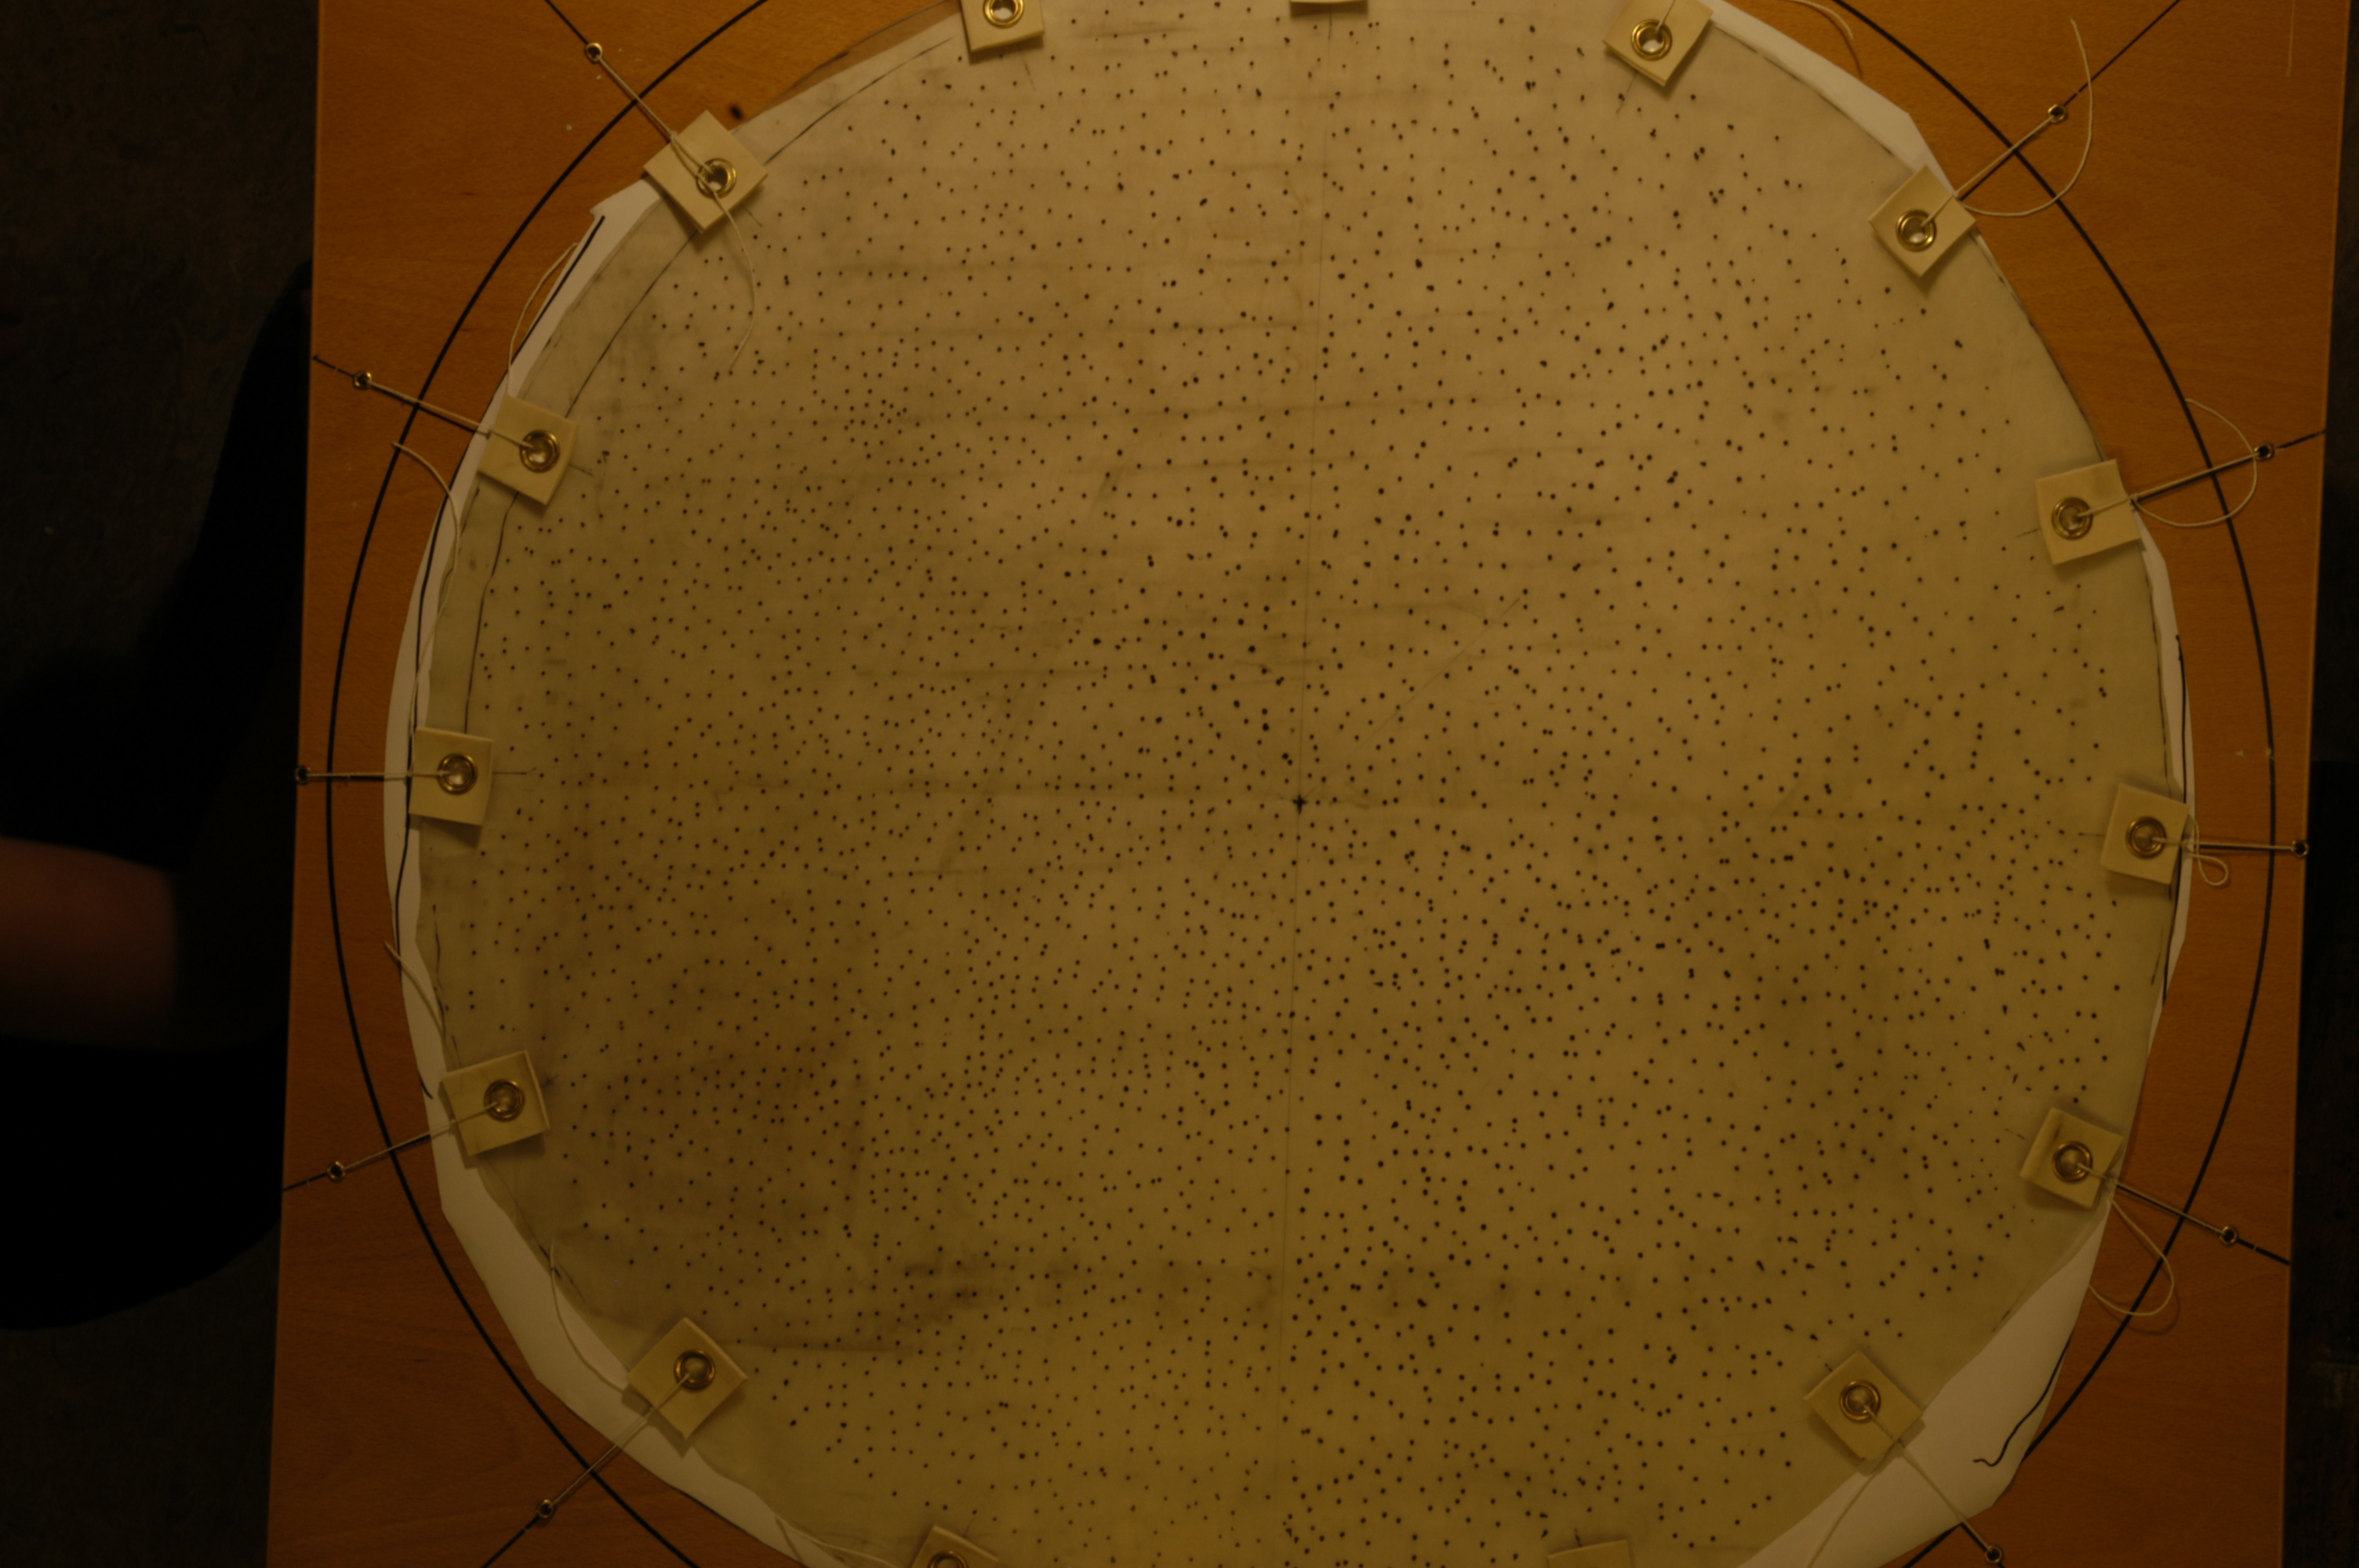
\includegraphics[scale=0.05]{PIC1.jpg} 
\caption{show an example picture}
\end{figure}
\end{frame}

\subsection{joining picture and lists} 

\begin{frame}
\frametitle{pictures and lists in beamer class}
\begin{columns}
\begin{column}{5cm}
\begin{itemize}
\item<1-> subject 1
\item<3-> subject 2
\item<5-> subject 3
\end{itemize}
\vspace{3cm} 
\end{column}
\begin{column}{5cm}
\begin{overprint}
\includegraphics<2>[scale=0.05]{PIC1.jpg}
\includegraphics<4>[scale=0.05]{PIC2.jpg}
\includegraphics<6>[scale=0.05]{PIC3.jpg}
\end{overprint}
\end{column}
\end{columns}
\end{frame}


\subsection{pictures which need more space} 
\begin{frame}[plain]
\frametitle{plain, or a way to get more space}
\begin{figure}
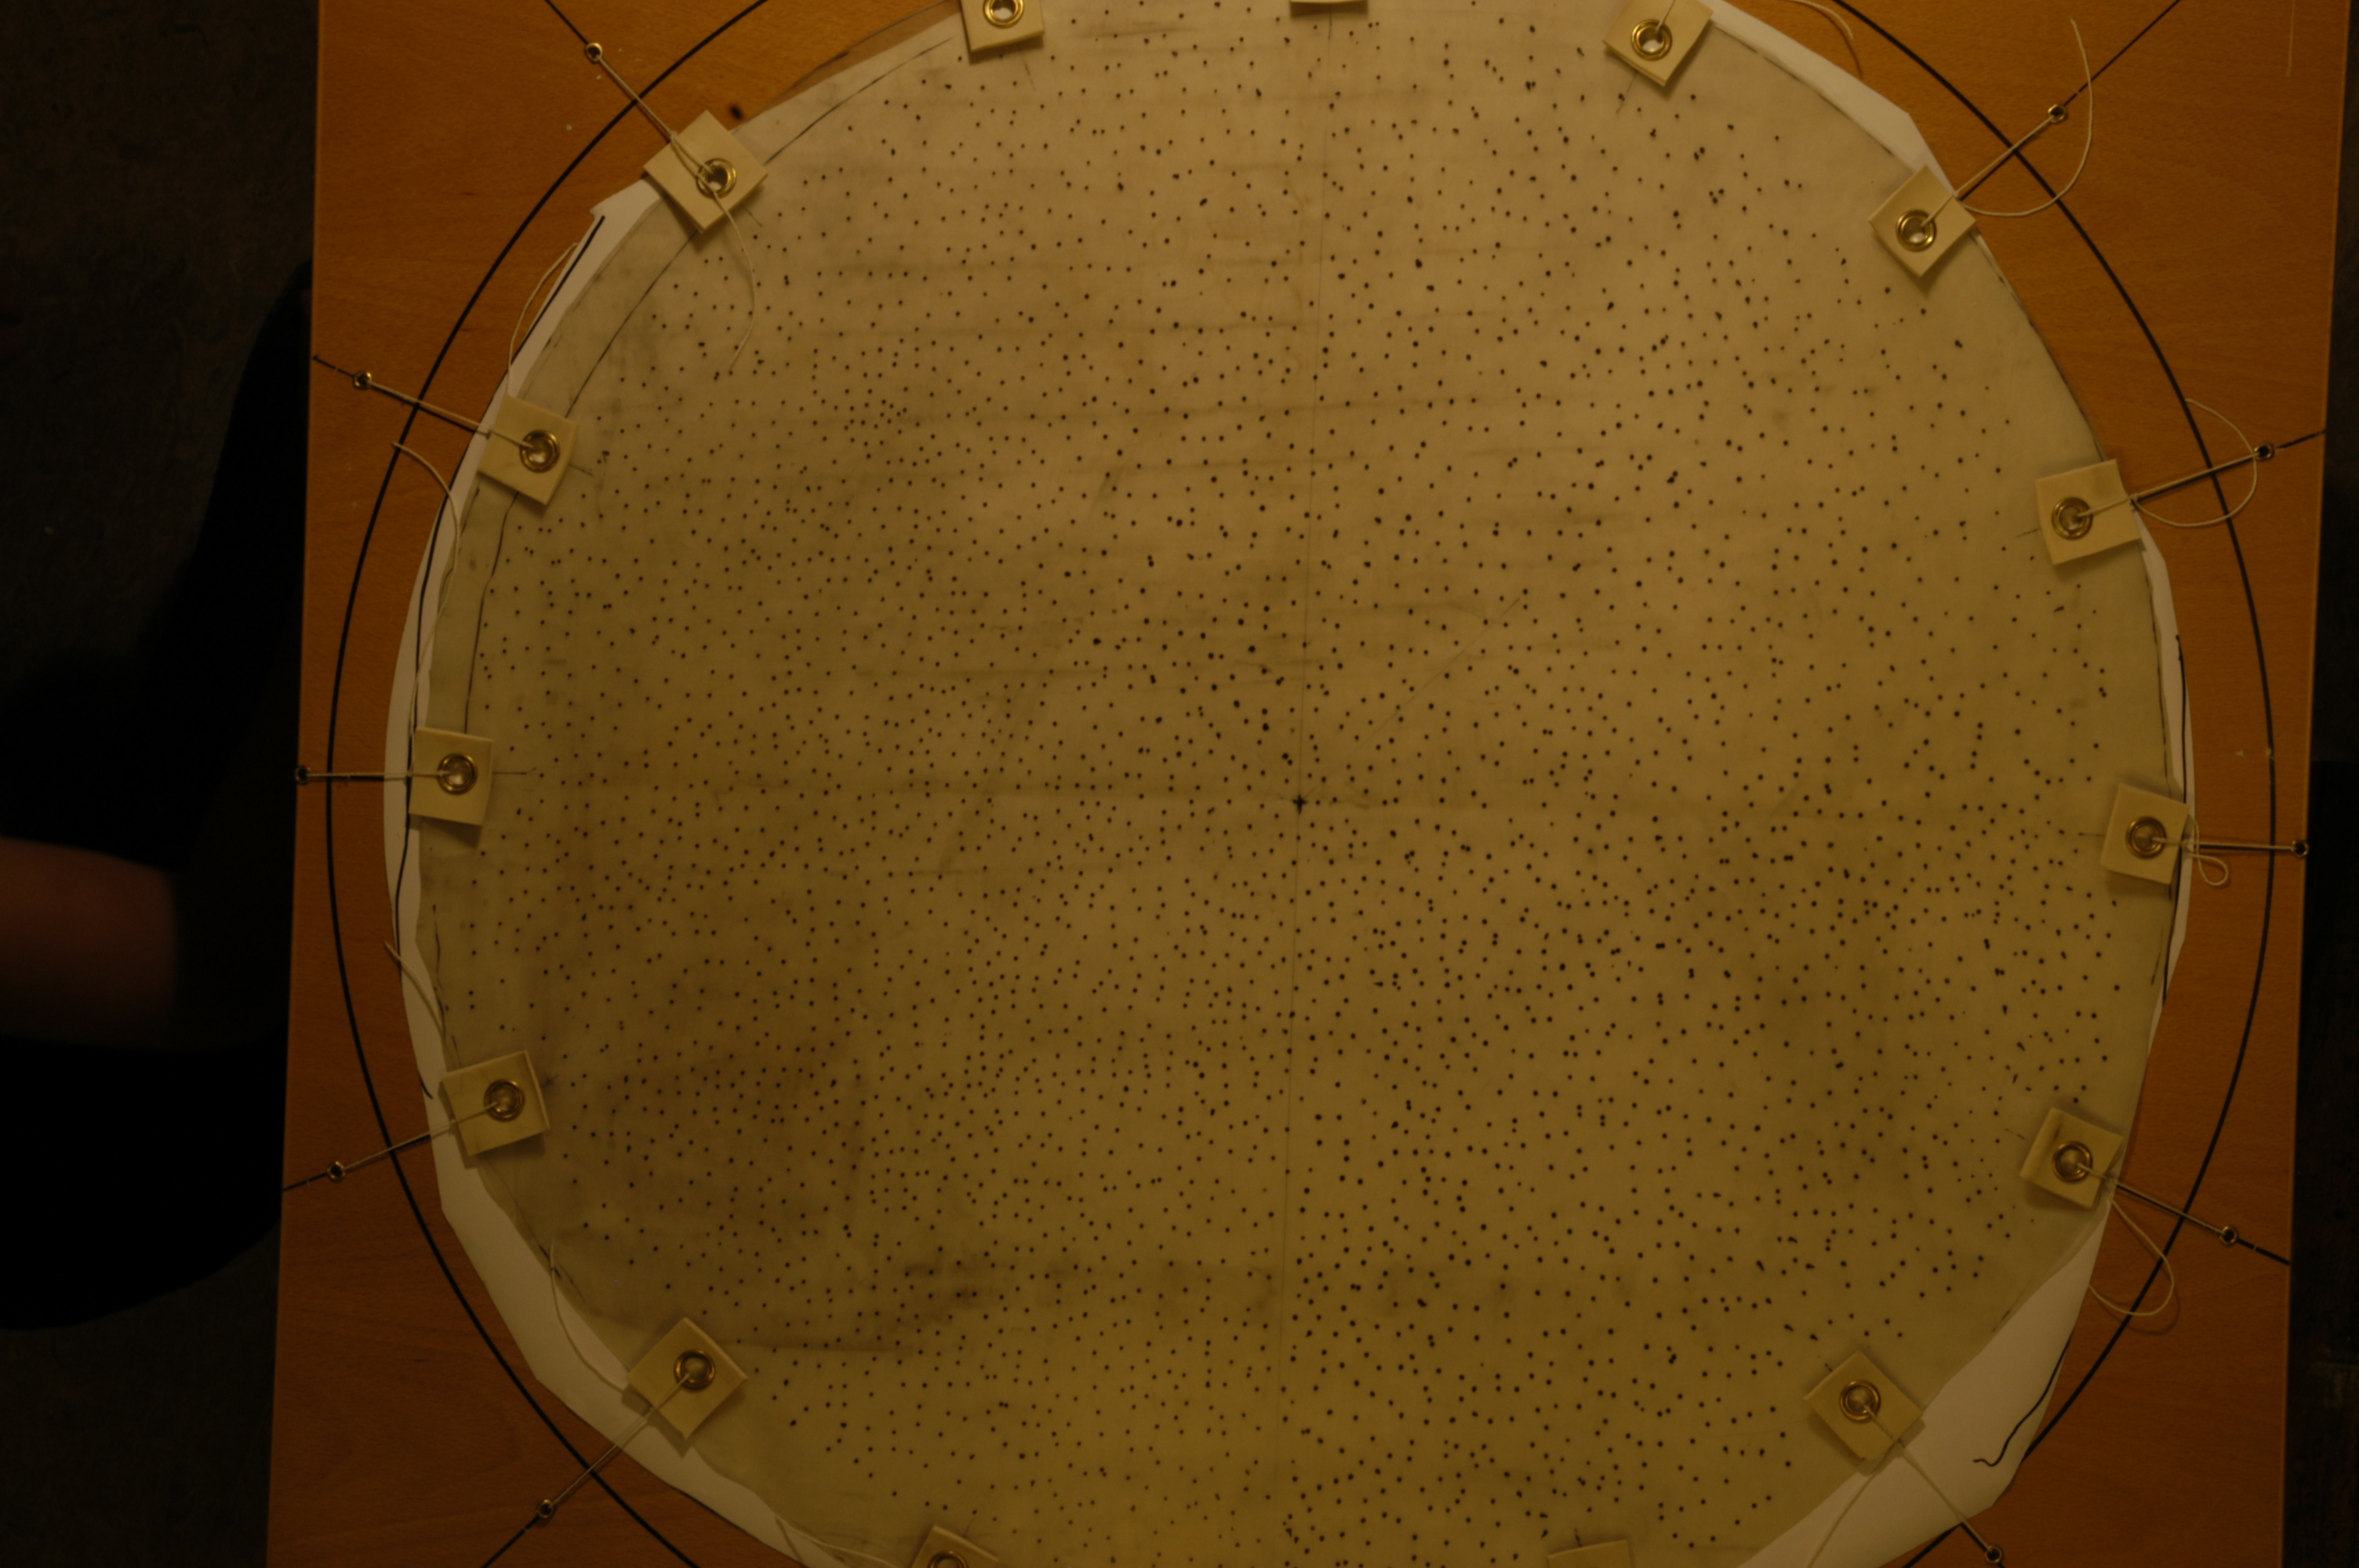
\includegraphics[scale=0.05]{PIC1.jpg} 
\caption{show an example picture}
\end{figure}
\end{frame}



\end{document}